\documentclass[aps,pra,showpacs,preprintnumbers,amsmath,amssymb,nofootinbib]{revtex4-2}
% \documentclass[aps,pra,showpacs,twocolumn,preprintnumbers,amsmath,amssymb,footinbib]{revtex4-2}

\usepackage{graphicx}
\usepackage{hyperref}
\usepackage{cleveref}
%\usepackage[mathlines]{lineno}% Enable numbering of text and display math
%\linenumbers\relax % Commence numbering lines

\usepackage[%showframe,%Uncomment any one of the following lines to test 
%scale=0.7, marginratio={1:1, 2:3}, ignoreall,% default settings
%text={7in,10in},centering,
%margin=1.5in,
%total={6.5in,8.75in}, top=1.2in, left=0.9in, includefoot,
%height=10in,a5paper,hmargin={3cm,0.8in},
]{geometry}
\usepackage{algorithm} 
\usepackage[noend]{algpseudocode}
\usepackage[caption=false]{subfig}

\usepackage{tikz}
\usepackage{pgfplots}
\usetikzlibrary{external}
% \usepgfplotslibrary{colormaps}
\tikzexternalize[prefix=plots/tmp/] % activate and define figures/ as cache folder


\def\CC{{C\nolinebreak[4]\hspace{-.05em}\raisebox{.4ex}{\tiny\bf ++}}}


\renewcommand{\bibsection}{%
  \par\mbox{}%
  \section*{References}%
}

\begin{document}
    % metadata
    \title{Report\\Exercise 2: Nagel-Schreckenberg-Model}
    \author{Tim Pokart}
     \email{tim.pokart@mailbox.tu-dresden.de}
     \affiliation{Technische Universität Dresden}
    \date{\today}
    
    \begin{abstract}
        In this short report the results from an exercise on the Nagel-Schreckenberg-model are presented, comparing our own implementation to the original \cite{NASC92} and the exercises \cite{SC22} results.
    \end{abstract}
        
    \maketitle

    \tableofcontents

    \section{Problem}

    We desire to study traffic flow with a focus on the appearance of congestion.
    For this we implement the Nagel-Schreckenberg-Model \cite{NASC92}.
    It models the road using a single-lane street of length $L > 100$ on which $N$ cars drive.
    Each of the cars occupies a discrete position $x \in \{1, \ldots, L\}$ and currently drives with velocity $v_i \in \{1,\ldots, v_{\mathrm{max}}\}$.
    In each iteration or time step with $t \in \mathbb{Z}$ of the model, we update the $i$\textsuperscript{th} cars position according to \cref{alg:nagel-schreckenberg-model}. 
    
    \begin{algorithm}[H]
        \caption{Nagel-Schreckenberg-Model}
        \label{alg:nagel-schreckenberg-model}
        \textbf{Input:} length $L$, cars $N$, positions $x_i$, velocities $v_i$\\
        \textbf{Parameter:} breaking probability $p$, maximum velocity $v_{\mathrm{max}}$

        \begin{algorithmic}[1]
            \Procedure{NagelSchreckenbergStep}{}
                \If {$v_i < v_{\mathrm{max}}$} \Comment{Accelerate}
                    \State $v_i \rightarrow v_i + 1$
                \EndIf

                \State $v_i \rightarrow \max (v_i, x_{i+1} - x_i - 1)$ \Comment{Avoid Collisions}
                \If {$v_i > 0$ \textbf{and} uniform random number $\in [0, 1] < p$} \Comment{Randomly decelerate}
                    \State $v_i \rightarrow v_i - 1$
                \EndIf

                \State $x_i \rightarrow x_i + v_i$ \Comment{Move}
            \EndProcedure
            \Statex
            \For{fixed amount of iterations} 
                \State \Call{NagelSchreckenbergStep}{}
            \EndFor
        \end{algorithmic}

    \end{algorithm}

    \section{Theoretical considerations}

    The velocity of a driver on a free road is given by his maximum velocity $v_{\mathrm{max}}$ and his accidental breaking probability $p$.
    In $1-p$ of the times, he drives with $v_{\mathrm{max}}$ and in $p$ of the times with $v_{\mathrm{max}} - 1$.
    His free velocity is therefore given by 
    \begin{align*}
        v_{\mathrm{free}} = (1 - p) v_{\mathrm{max}} + p (v_{\mathrm{max}} - 1) = v_{\mathrm{max}} - p.
    \end{align*}

    We want to quantify the flow \[Q = N / T\] with the time $T$ it takes one car  to travel along the whole road on average. 
    In order to calculate it we use the cars velocities according to
    \begin{align*}
        Q = \frac{N}{T} = \frac{N}{L} \frac{L}{T} = \frac{1}{L} \sum_i \frac{L}{t_i} = \frac{1}{L} \sum_i v_i
    \end{align*}
    with $t_i$ the time it would take the $i$\textsuperscript{th} car to travel along.

    \section{Results and Discussion}

    We chose $L = 1000$\footnote{We had to resort to $L = 400$ for the space-time-plots in order to be able to employ inline-\LaTeX{} rendering with pgfplots, since the \LaTeX{} compiler is utterly inefficient but the authors insisted on using it.} and define the car density $\rho = N / L$.
    Each car is placed randomly on the road and assigned a $v = 0$ velocity.

    Comparing to the reference material, we find that both the flow-density relationship and the space-time-plots exhibit the expected behaviour.
    Namely
    \begin{itemize}
        \item the flow-density-relationship for both $v_{\mathrm{max}} = 1$ and $v_{\mathrm{max}} = 5$ increase until the density gets to high, frequent and large-scale congestion occurs and the overall flow $Q$ decreases.
        \item The space-time-plots show moving congestions which increase in severity with increasing breaking probability.
    \end{itemize}
   
    We furthermore notice the following: The congestions for $v_{\mathrm{max}} = 5$ dissolve in a fascinating pattern.
    Each congestions moves slowly with the traffic, however its ends curve in the opposite direction and move against the traffic.
    This could for example be caused by a driver close to the congestion breaking by chance and accidentally breaking up the congestion. 


    \begin{figure}[H]
        \subfloat[$v_{\mathrm{max}} = 1$]{\begin{tikzpicture}
    \begin{axis}[ xmin=0, xmax=0.6, ymin=0, ymax=0.2, xlabel={density $\rho$}, ylabel={flow $Q$}, ytick={0,0.05,0.1,0.15,0.2}, yticklabels={0,0.05,0.1,0.15,0.2}, legend cell align={left} ]
        \addplot[only marks, mark=*,mark options={fill=teal}] table[x=RHO,y expr=1/(5-0.05)*\thisrow{Q},col sep=semicolon] {plots/vmax5/flow_0_05.csv};
        \addplot[only marks, mark=pentagon*,mark options={fill=violet}] table[x=RHO,y expr=1/(5-0.2)*\thisrow{Q},col sep=semicolon] {plots/vmax5/flow_0_2.csv};
        \addplot[only marks, mark=square*,mark options={fill=purple}] table[x=RHO,y expr=1/(5-0.35)*\thisrow{Q},col sep=semicolon] {plots/vmax5/flow_0_35.csv};
        
        \addplot[domain=0:1, samples=10, thick, dashed] {x};
        \path [thick] (axis cs:0,0) -- (axis cs:0.2,0.2) node[above, near end, sloped] { $Q = \rho v_{\mathrm{free}}$ };

        \legend{$p=0.05$, $p=0.2$, $p=0.35$};
    \end{axis}
\end{tikzpicture}
}
        \subfloat[$v_{\mathrm{max}} = 5$]{\begin{tikzpicture}
    \begin{axis}[ xmin=0, xmax=0.6, ymin=0, ymax=0.2, xlabel={density $\rho$}, ylabel={flow $Q$}, ytick={0,0.05,0.1,0.15,0.2}, yticklabels={0,0.05,0.1,0.15,0.2}, legend cell align={left} ]
        \addplot[only marks, mark=*,mark options={fill=teal}] table[x=RHO,y expr=1/(5-0.05)*\thisrow{Q},col sep=semicolon] {plots/vmax5/flow_0_05.csv};
        \addplot[only marks, mark=pentagon*,mark options={fill=violet}] table[x=RHO,y expr=1/(5-0.2)*\thisrow{Q},col sep=semicolon] {plots/vmax5/flow_0_2.csv};
        \addplot[only marks, mark=square*,mark options={fill=purple}] table[x=RHO,y expr=1/(5-0.35)*\thisrow{Q},col sep=semicolon] {plots/vmax5/flow_0_35.csv};
        
        \addplot[domain=0:1, samples=10, thick, dashed] {x};
        \path [thick] (axis cs:0,0) -- (axis cs:0.2,0.2) node[above, near end, sloped] { $Q = \rho v_{\mathrm{free}}$ };

        \legend{$p=0.05$, $p=0.2$, $p=0.35$};
    \end{axis}
\end{tikzpicture}
}
        \caption{Flow-density-relationship for respective maximum velocities.}
    \end{figure}
    
    \section{Extensions}
    
    One extension which could be implemented is to allow for further acceleration beyong the $v_{\mathrm{max}}$ limit. 
    We implemented a probabilistic acceleration curve in which a driver above $v_{\mathrm{max}}$ accelerates according to the changes given in \cref{fig:extension:2}.
    Noteably, the maximum flow decreases, despite the free velocity increasing significantly (from $v_{\mathrm{free}} = 4.65$ to $v_{\mathrm{free}} = 5.38$ with further acceleration\footnote{The free velocity was obtained from a numerical simulation}). 

    \begin{figure}[H]
        \subfloat{
            \begin{tikzpicture}
                \begin{axis}[ xmin=0, xmax=0.2, ymin=0, xlabel={density $\rho$}, ylabel={normalized flow $Q / v_{\mathrm{free}}$}, legend cell align={left}, xtick={0,0.05,0.1,0.15,0.2}, width=0.45\linewidth, legend style={at={(axis cs:0.195,0.01)},anchor=south east}, tick label style={/pgf/number format/fixed}]
                    \addplot[only marks, mark size=1pt, mark=*,mark options={fill=teal}] table[x=RHO,y expr=\thisrow{Q} / 5.38,col sep=semicolon] {plots/vmax5/flow_0_35_exp_highres.csv};
                    \addplot[only marks, mark size=1pt, mark=square*,mark options={fill=purple}] table[x=RHO,y expr=\thisrow{Q} / 4.65,col sep=semicolon] {plots/vmax5/flow_0_35_highres.csv};
                    
                    \legend{with further acceleration, without further acceleration}
                \end{axis}
            \end{tikzpicture}\label{fig:extension:1} 
        }
        \subfloat{
            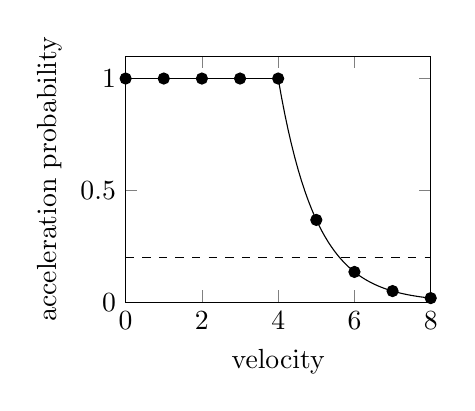
\begin{tikzpicture}
                \begin{axis}[xmin=0, xmax=8, domain=0:10, ymax=1.1, ymin=0, ylabel={acceleration probability}, xlabel={velocity}, width=0.45\linewidth]
                    \addplot[only marks, samples=11] {min(1.0, exp(-(x-4)))};
                    \addplot[samples=10, domain=0:4] {min(1.0, exp(-(x-4)))};
                    \addplot[samples=70, domain=4:10] {min(1.0, exp(-(x-4)))};
                    \addplot[samples=10, dashed] {0.2};
                \end{axis}
            \end{tikzpicture}\label{fig:extension:2}
        }
        \caption{Density-flow-chart and acceleration probability of the implemented extension.}
    \end{figure}

    \begin{acknowledgments}
        We wish to acknowledge Malte Schröder for posing such an interesting question, providing the data and reading through this report. 
    \end{acknowledgments}

    \appendix
    
    \section{Space-time plots}
    \begin{figure}[H]
        \subfloat[$\rho = 0.05$]{\begin{tikzpicture}
    \pgfplotsset{
        % this *defines* a custom colormap ...
        colormap={inferno}{
            rgb255=(0,0,4)
            rgb255=(12,8,38)
            rgb255=(36,12,79)
            rgb255=(66,10,104)
            rgb255=(93,18,110)
            rgb255=(120,28,109)
            rgb255=(147,38,103)
            rgb255=(174,48,92)
            rgb255=(199,62,76)
            rgb255=(221,81,58)
            rgb255=(237,105,37)
            rgb255=(248,133,15)
            rgb255=(252,165,10)
            rgb255=(250,198,45)
            rgb255=(242,230,97)
            rgb255=(252,255,164)
        }
    }
    \begin{axis}[
            view={0}{90},
            xlabel={$t$},
            ylabel={position $i$},
            colormap={CM}{
                % name = inferno
                samples of colormap=(6 of inferno)
            },
            colorbar sampled,
            colormap access=piecewise constant,
            point meta min=0,
            point meta max=6,
            colorbar right,
            colorbar style={%
                ytick=data,
                samples=7,
                title=$v$,
                ytick = {0,1,2,3,4,5,6},
                ymax=6,
                ymin=0,
                yticklabels ={
                    \raisebox{9mm}{0}, 
                    \raisebox{9mm}{1}, 
                    \raisebox{9mm}{2}, 
                    \raisebox{9mm}{3}, 
                    \raisebox{9mm}{4}, 
                    \raisebox{9mm}{5}, 
                    \raisebox{9mm}{$ $} }
            },
            enlargelimits=0,
            width=.4\textwidth
        ]
        \addplot[scatter, only marks, mark options={scale=0.5}, point meta=explicit] table[x=T,y=P, meta=V, col sep=semicolon] {plots/tpv_rho_0_05_p_0_05.csv};
    \end{axis}
\end{tikzpicture}}
        \subfloat[$\rho = 0.15$]{\begin{tikzpicture}
    \pgfplotsset{
        % this *defines* a custom colormap ...
        colormap={inferno}{
            rgb255=(0,0,4)
            rgb255=(12,8,38)
            rgb255=(36,12,79)
            rgb255=(66,10,104)
            rgb255=(93,18,110)
            rgb255=(120,28,109)
            rgb255=(147,38,103)
            rgb255=(174,48,92)
            rgb255=(199,62,76)
            rgb255=(221,81,58)
            rgb255=(237,105,37)
            rgb255=(248,133,15)
            rgb255=(252,165,10)
            rgb255=(250,198,45)
            rgb255=(242,230,97)
            rgb255=(252,255,164)
        }
    }
    \begin{axis}[
            view={0}{90},
            xlabel={$t$},
            ylabel={position $i$},
            colormap={CM}{
                % name = inferno
                samples of colormap=(6 of inferno)
            },
            colorbar sampled,
            colormap access=piecewise constant,
            point meta min=0,
            point meta max=6,
            colorbar right,
            colorbar style={%
                ytick=data,
                samples=7,
                title=$v$,
                ytick = {0,1,2,3,4,5,6},
                ymax=6,
                ymin=0,
                yticklabels ={
                    \raisebox{9mm}{0}, 
                    \raisebox{9mm}{1}, 
                    \raisebox{9mm}{2}, 
                    \raisebox{9mm}{3}, 
                    \raisebox{9mm}{4}, 
                    \raisebox{9mm}{5}, 
                    \raisebox{9mm}{$ $} }
            },
            enlargelimits=0,
            width=.4\textwidth
        ]
        \addplot[scatter, only marks, mark options={scale=0.5}, point meta=explicit] table[x=T,y=P, meta=V, col sep=semicolon] {plots/tpv_rho_0_15_p_0_05.csv};
    \end{axis}
\end{tikzpicture}} \\
        \subfloat[$\rho = 0.25$]{\begin{tikzpicture}
    \pgfplotsset{
        % this *defines* a custom colormap ...
        colormap={inferno}{
            rgb255=(0,0,4)
            rgb255=(12,8,38)
            rgb255=(36,12,79)
            rgb255=(66,10,104)
            rgb255=(93,18,110)
            rgb255=(120,28,109)
            rgb255=(147,38,103)
            rgb255=(174,48,92)
            rgb255=(199,62,76)
            rgb255=(221,81,58)
            rgb255=(237,105,37)
            rgb255=(248,133,15)
            rgb255=(252,165,10)
            rgb255=(250,198,45)
            rgb255=(242,230,97)
            rgb255=(252,255,164)
        }
    }
    \begin{axis}[
            view={0}{90},
            xlabel={$t$},
            ylabel={position $i$},
            colormap={CM}{
                % name = inferno
                samples of colormap=(6 of inferno)
            },
            colorbar sampled,
            colormap access=piecewise constant,
            point meta min=0,
            point meta max=6,
            colorbar right,
            colorbar style={%
                ytick=data,
                samples=7,
                title=$v$,
                ytick = {0,1,2,3,4,5,6},
                ymax=6,
                ymin=0,
                yticklabels ={
                    \raisebox{9mm}{0}, 
                    \raisebox{9mm}{1}, 
                    \raisebox{9mm}{2}, 
                    \raisebox{9mm}{3}, 
                    \raisebox{9mm}{4}, 
                    \raisebox{9mm}{5}, 
                    \raisebox{9mm}{$ $} }
            },
            enlargelimits=0,
            width=.4\textwidth
        ]
        \addplot[scatter, only marks, mark options={scale=0.5}, point meta=explicit] table[x=T,y=P, meta=V, col sep=semicolon] {plots/tpv_rho_0_25_p_0_05.csv};
    \end{axis}
\end{tikzpicture}}
        \caption{car dynamics with $v_{\mathrm{max}} = 1$ in a space-time-plot with breaking probability $p = 0.05$.}
    \end{figure}
    
    \begin{figure}[H]
        \subfloat[$\rho = 0.05$]{\begin{tikzpicture}
    \pgfplotsset{
        % this *defines* a custom colormap ...
        colormap={inferno}{
            rgb255=(0,0,4)
            rgb255=(12,8,38)
            rgb255=(36,12,79)
            rgb255=(66,10,104)
            rgb255=(93,18,110)
            rgb255=(120,28,109)
            rgb255=(147,38,103)
            rgb255=(174,48,92)
            rgb255=(199,62,76)
            rgb255=(221,81,58)
            rgb255=(237,105,37)
            rgb255=(248,133,15)
            rgb255=(252,165,10)
            rgb255=(250,198,45)
            rgb255=(242,230,97)
            rgb255=(252,255,164)
        }
    }
    \begin{axis}[
            view={0}{90},
            xlabel={$t$},
            ylabel={position $i$},
            colormap={CM}{
                % name = inferno
                samples of colormap=(6 of inferno)
            },
            colorbar sampled,
            colormap access=piecewise constant,
            point meta min=0,
            point meta max=6,
            colorbar right,
            colorbar style={%
                ytick=data,
                samples=7,
                title=$v$,
                ytick = {0,1,2,3,4,5,6},
                ymax=6,
                ymin=0,
                yticklabels ={
                    \raisebox{9mm}{0}, 
                    \raisebox{9mm}{1}, 
                    \raisebox{9mm}{2}, 
                    \raisebox{9mm}{3}, 
                    \raisebox{9mm}{4}, 
                    \raisebox{9mm}{5}, 
                    \raisebox{9mm}{$ $} }
            },
            enlargelimits=0,
            width=.4\textwidth
        ]
        \addplot[scatter, only marks, mark options={scale=0.5}, point meta=explicit] table[x=T,y=P, meta=V, col sep=semicolon] {plots/tpv_rho_0_05_p_0_20.csv};
    \end{axis}
\end{tikzpicture}}
        \subfloat[$\rho = 0.15$]{\begin{tikzpicture}
    \pgfplotsset{
        % this *defines* a custom colormap ...
        colormap={inferno}{
            rgb255=(0,0,4)
            rgb255=(12,8,38)
            rgb255=(36,12,79)
            rgb255=(66,10,104)
            rgb255=(93,18,110)
            rgb255=(120,28,109)
            rgb255=(147,38,103)
            rgb255=(174,48,92)
            rgb255=(199,62,76)
            rgb255=(221,81,58)
            rgb255=(237,105,37)
            rgb255=(248,133,15)
            rgb255=(252,165,10)
            rgb255=(250,198,45)
            rgb255=(242,230,97)
            rgb255=(252,255,164)
        }
    }
    \begin{axis}[
            view={0}{90},
            xlabel={$t$},
            ylabel={position $i$},
            colormap={CM}{
                % name = inferno
                samples of colormap=(6 of inferno)
            },
            colorbar sampled,
            colormap access=piecewise constant,
            point meta min=0,
            point meta max=6,
            colorbar right,
            colorbar style={%
                ytick=data,
                samples=7,
                title=$v$,
                ytick = {0,1,2,3,4,5,6},
                ymax=6,
                ymin=0,
                yticklabels ={
                    \raisebox{9mm}{0}, 
                    \raisebox{9mm}{1}, 
                    \raisebox{9mm}{2}, 
                    \raisebox{9mm}{3}, 
                    \raisebox{9mm}{4}, 
                    \raisebox{9mm}{5}, 
                    \raisebox{9mm}{$ $} }
            },
            enlargelimits=0,
            width=.4\textwidth
        ]
        \addplot[scatter, only marks, mark options={scale=0.5}, point meta=explicit] table[x=T,y=P, meta=V, col sep=semicolon] {plots/tpv_rho_0_15_p_0_20.csv};
    \end{axis}
\end{tikzpicture}} \\
        \subfloat[$\rho = 0.25$]{\begin{tikzpicture}
    \pgfplotsset{
        % this *defines* a custom colormap ...
        colormap={inferno}{
            rgb255=(0,0,4)
            rgb255=(12,8,38)
            rgb255=(36,12,79)
            rgb255=(66,10,104)
            rgb255=(93,18,110)
            rgb255=(120,28,109)
            rgb255=(147,38,103)
            rgb255=(174,48,92)
            rgb255=(199,62,76)
            rgb255=(221,81,58)
            rgb255=(237,105,37)
            rgb255=(248,133,15)
            rgb255=(252,165,10)
            rgb255=(250,198,45)
            rgb255=(242,230,97)
            rgb255=(252,255,164)
        }
    }
    \begin{axis}[
            view={0}{90},
            xlabel={$t$},
            ylabel={position $i$},
            colormap={CM}{
                % name = inferno
                samples of colormap=(6 of inferno)
            },
            colorbar sampled,
            colormap access=piecewise constant,
            point meta min=0,
            point meta max=6,
            colorbar right,
            colorbar style={%
                ytick=data,
                samples=7,
                title=$v$,
                ytick = {0,1,2,3,4,5,6},
                ymax=6,
                ymin=0,
                yticklabels ={
                    \raisebox{9mm}{0}, 
                    \raisebox{9mm}{1}, 
                    \raisebox{9mm}{2}, 
                    \raisebox{9mm}{3}, 
                    \raisebox{9mm}{4}, 
                    \raisebox{9mm}{5}, 
                    \raisebox{9mm}{$ $} }
            },
            enlargelimits=0,
            width=.4\textwidth
        ]
        \addplot[scatter, only marks, mark options={scale=0.5}, point meta=explicit] table[x=T,y=P, meta=V, col sep=semicolon] {plots/tpv_rho_0_25_p_0_20.csv};
    \end{axis}
\end{tikzpicture}}
        \caption{car dynamics with $v_{\mathrm{max}} = 1$ in a space-time-plot with breaking probability $p = 0.20$.}
    \end{figure}
    
    \begin{figure}[H]
        \subfloat[$\rho = 0.05$]{\begin{tikzpicture}
    \pgfplotsset{
        % this *defines* a custom colormap ...
        colormap={inferno}{
            rgb255=(0,0,4)
            rgb255=(12,8,38)
            rgb255=(36,12,79)
            rgb255=(66,10,104)
            rgb255=(93,18,110)
            rgb255=(120,28,109)
            rgb255=(147,38,103)
            rgb255=(174,48,92)
            rgb255=(199,62,76)
            rgb255=(221,81,58)
            rgb255=(237,105,37)
            rgb255=(248,133,15)
            rgb255=(252,165,10)
            rgb255=(250,198,45)
            rgb255=(242,230,97)
            rgb255=(252,255,164)
        }
    }
    \begin{axis}[
            view={0}{90},
            xlabel={$t$},
            ylabel={position $i$},
            colormap={CM}{
                % name = inferno
                samples of colormap=(6 of inferno)
            },
            colorbar sampled,
            colormap access=piecewise constant,
            point meta min=0,
            point meta max=6,
            colorbar right,
            colorbar style={%
                ytick=data,
                samples=7,
                title=$v$,
                ytick = {0,1,2,3,4,5,6},
                ymax=6,
                ymin=0,
                yticklabels ={
                    \raisebox{9mm}{0}, 
                    \raisebox{9mm}{1}, 
                    \raisebox{9mm}{2}, 
                    \raisebox{9mm}{3}, 
                    \raisebox{9mm}{4}, 
                    \raisebox{9mm}{5}, 
                    \raisebox{9mm}{$ $} }
            },
            enlargelimits=0,
            width=.4\textwidth
        ]
        \addplot[scatter, only marks, mark options={scale=0.5}, point meta=explicit] table[x=T,y=P, meta=V, col sep=semicolon] {plots/tpv_rho_0_05_p_0_35.csv};
    \end{axis}
\end{tikzpicture}}
        \subfloat[$\rho = 0.15$]{\begin{tikzpicture}
    \pgfplotsset{
        % this *defines* a custom colormap ...
        colormap={inferno}{
            rgb255=(0,0,4)
            rgb255=(12,8,38)
            rgb255=(36,12,79)
            rgb255=(66,10,104)
            rgb255=(93,18,110)
            rgb255=(120,28,109)
            rgb255=(147,38,103)
            rgb255=(174,48,92)
            rgb255=(199,62,76)
            rgb255=(221,81,58)
            rgb255=(237,105,37)
            rgb255=(248,133,15)
            rgb255=(252,165,10)
            rgb255=(250,198,45)
            rgb255=(242,230,97)
            rgb255=(252,255,164)
        }
    }
    \begin{axis}[
            view={0}{90},
            xlabel={$t$},
            ylabel={position $i$},
            colormap={CM}{
                % name = inferno
                samples of colormap=(6 of inferno)
            },
            colorbar sampled,
            colormap access=piecewise constant,
            point meta min=0,
            point meta max=6,
            colorbar right,
            colorbar style={%
                ytick=data,
                samples=7,
                title=$v$,
                ytick = {0,1,2,3,4,5,6},
                ymax=6,
                ymin=0,
                yticklabels ={
                    \raisebox{9mm}{0}, 
                    \raisebox{9mm}{1}, 
                    \raisebox{9mm}{2}, 
                    \raisebox{9mm}{3}, 
                    \raisebox{9mm}{4}, 
                    \raisebox{9mm}{5}, 
                    \raisebox{9mm}{$ $} }
            },
            enlargelimits=0,
            width=.4\textwidth
        ]
        \addplot[scatter, only marks, mark options={scale=0.5}, point meta=explicit] table[x=T,y=P, meta=V, col sep=semicolon] {plots/tpv_rho_0_15_p_0_35.csv};
    \end{axis}
\end{tikzpicture}} \\
        \subfloat[$\rho = 0.25$]{\begin{tikzpicture}
    \pgfplotsset{
        % this *defines* a custom colormap ...
        colormap={inferno}{
            rgb255=(0,0,4)
            rgb255=(12,8,38)
            rgb255=(36,12,79)
            rgb255=(66,10,104)
            rgb255=(93,18,110)
            rgb255=(120,28,109)
            rgb255=(147,38,103)
            rgb255=(174,48,92)
            rgb255=(199,62,76)
            rgb255=(221,81,58)
            rgb255=(237,105,37)
            rgb255=(248,133,15)
            rgb255=(252,165,10)
            rgb255=(250,198,45)
            rgb255=(242,230,97)
            rgb255=(252,255,164)
        }
    }
    \begin{axis}[
            view={0}{90},
            xlabel={$t$},
            ylabel={position $i$},
            colormap={CM}{
                % name = inferno
                samples of colormap=(6 of inferno)
            },
            colorbar sampled,
            colormap access=piecewise constant,
            point meta min=0,
            point meta max=6,
            colorbar right,
            colorbar style={%
                ytick=data,
                samples=7,
                title=$v$,
                ytick = {0,1,2,3,4,5,6},
                ymax=6,
                ymin=0,
                yticklabels ={
                    \raisebox{9mm}{0}, 
                    \raisebox{9mm}{1}, 
                    \raisebox{9mm}{2}, 
                    \raisebox{9mm}{3}, 
                    \raisebox{9mm}{4}, 
                    \raisebox{9mm}{5}, 
                    \raisebox{9mm}{$ $} }
            },
            enlargelimits=0,
            width=.4\textwidth
        ]
        \addplot[scatter, only marks, mark options={scale=0.5}, point meta=explicit] table[x=T,y=P, meta=V, col sep=semicolon] {plots/tpv_rho_0_25_p_0_35.csv};
    \end{axis}
\end{tikzpicture}}
        \caption{car dynamics with $v_{\mathrm{max}} = 1$ in a space-time-plot with breaking probability $p = 0.35$.}
    \end{figure}
    
    \begin{figure}[H]
        \subfloat[$\rho = 0.05$]{\begin{tikzpicture}
    \pgfplotsset{
        % this *defines* a custom colormap ...
        colormap={inferno}{
            rgb255=(0,0,4)
            rgb255=(12,8,38)
            rgb255=(36,12,79)
            rgb255=(66,10,104)
            rgb255=(93,18,110)
            rgb255=(120,28,109)
            rgb255=(147,38,103)
            rgb255=(174,48,92)
            rgb255=(199,62,76)
            rgb255=(221,81,58)
            rgb255=(237,105,37)
            rgb255=(248,133,15)
            rgb255=(252,165,10)
            rgb255=(250,198,45)
            rgb255=(242,230,97)
            rgb255=(252,255,164)
        }
    }
    \begin{axis}[
            view={0}{90},
            xlabel={$t$},
            ylabel={position $i$},
            colormap={CM}{
                % name = inferno
                samples of colormap=(6 of inferno)
            },
            colorbar sampled,
            colormap access=piecewise constant,
            point meta min=0,
            point meta max=6,
            colorbar right,
            colorbar style={%
                ytick=data,
                samples=7,
                title=$v$,
                ytick = {0,1,2,3,4,5,6},
                ymax=6,
                ymin=0,
                yticklabels ={
                    \raisebox{9mm}{0}, 
                    \raisebox{9mm}{1}, 
                    \raisebox{9mm}{2}, 
                    \raisebox{9mm}{3}, 
                    \raisebox{9mm}{4}, 
                    \raisebox{9mm}{5}, 
                    \raisebox{9mm}{$ $} }
            },
            enlargelimits=0,
            width=.4\textwidth
        ]
        \addplot[scatter, only marks, mark options={scale=0.5}, point meta=explicit] table[x=T,y=P, meta=V, col sep=semicolon] {plots/vmax5/tpv_v5_rho_0_05_p_0_05.csv};
    \end{axis}
\end{tikzpicture}}
        \subfloat[$\rho = 0.15$]{\begin{tikzpicture}
    \pgfplotsset{
        % this *defines* a custom colormap ...
        colormap={inferno}{
            rgb255=(0,0,4)
            rgb255=(12,8,38)
            rgb255=(36,12,79)
            rgb255=(66,10,104)
            rgb255=(93,18,110)
            rgb255=(120,28,109)
            rgb255=(147,38,103)
            rgb255=(174,48,92)
            rgb255=(199,62,76)
            rgb255=(221,81,58)
            rgb255=(237,105,37)
            rgb255=(248,133,15)
            rgb255=(252,165,10)
            rgb255=(250,198,45)
            rgb255=(242,230,97)
            rgb255=(252,255,164)
        }
    }
    \begin{axis}[
            view={0}{90},
            xlabel={$t$},
            ylabel={position $i$},
            colormap={CM}{
                % name = inferno
                samples of colormap=(6 of inferno)
            },
            colorbar sampled,
            colormap access=piecewise constant,
            point meta min=0,
            point meta max=6,
            colorbar right,
            colorbar style={%
                ytick=data,
                samples=7,
                title=$v$,
                ytick = {0,1,2,3,4,5,6},
                ymax=6,
                ymin=0,
                yticklabels ={
                    \raisebox{9mm}{0}, 
                    \raisebox{9mm}{1}, 
                    \raisebox{9mm}{2}, 
                    \raisebox{9mm}{3}, 
                    \raisebox{9mm}{4}, 
                    \raisebox{9mm}{5}, 
                    \raisebox{9mm}{$ $} }
            },
            enlargelimits=0,
            width=.4\textwidth
        ]
        \addplot[scatter, only marks, mark options={scale=0.5}, point meta=explicit] table[x=T,y=P, meta=V, col sep=semicolon] {plots/vmax5/tpv_v5_rho_0_15_p_0_05.csv};
    \end{axis}
\end{tikzpicture}} \\
        \subfloat[$\rho = 0.25$]{\begin{tikzpicture}
    \pgfplotsset{
        % this *defines* a custom colormap ...
        colormap={inferno}{
            rgb255=(0,0,4)
            rgb255=(12,8,38)
            rgb255=(36,12,79)
            rgb255=(66,10,104)
            rgb255=(93,18,110)
            rgb255=(120,28,109)
            rgb255=(147,38,103)
            rgb255=(174,48,92)
            rgb255=(199,62,76)
            rgb255=(221,81,58)
            rgb255=(237,105,37)
            rgb255=(248,133,15)
            rgb255=(252,165,10)
            rgb255=(250,198,45)
            rgb255=(242,230,97)
            rgb255=(252,255,164)
        }
    }
    \begin{axis}[
            view={0}{90},
            xlabel={$t$},
            ylabel={position $i$},
            colormap={CM}{
                % name = inferno
                samples of colormap=(6 of inferno)
            },
            colorbar sampled,
            colormap access=piecewise constant,
            point meta min=0,
            point meta max=6,
            colorbar right,
            colorbar style={%
                ytick=data,
                samples=7,
                title=$v$,
                ytick = {0,1,2,3,4,5,6},
                ymax=6,
                ymin=0,
                yticklabels ={
                    \raisebox{9mm}{0}, 
                    \raisebox{9mm}{1}, 
                    \raisebox{9mm}{2}, 
                    \raisebox{9mm}{3}, 
                    \raisebox{9mm}{4}, 
                    \raisebox{9mm}{5}, 
                    \raisebox{9mm}{$ $} }
            },
            enlargelimits=0,
            width=.4\textwidth
        ]
        \addplot[scatter, only marks, mark options={scale=0.5}, point meta=explicit] table[x=T,y=P, meta=V, col sep=semicolon] {plots/vmax5/tpv_v5_rho_0_25_p_0_05.csv};
    \end{axis}
\end{tikzpicture}}
        \caption{car dynamics with $v_{\mathrm{max}} = 5$ in a space-time-plot with breaking probability $p = 0.05$.}
    \end{figure}
    
    \begin{figure}[H]
        \subfloat[$\rho = 0.05$]{\begin{tikzpicture}
    \pgfplotsset{
        % this *defines* a custom colormap ...
        colormap={inferno}{
            rgb255=(0,0,4)
            rgb255=(12,8,38)
            rgb255=(36,12,79)
            rgb255=(66,10,104)
            rgb255=(93,18,110)
            rgb255=(120,28,109)
            rgb255=(147,38,103)
            rgb255=(174,48,92)
            rgb255=(199,62,76)
            rgb255=(221,81,58)
            rgb255=(237,105,37)
            rgb255=(248,133,15)
            rgb255=(252,165,10)
            rgb255=(250,198,45)
            rgb255=(242,230,97)
            rgb255=(252,255,164)
        }
    }
    \begin{axis}[
            view={0}{90},
            xlabel={$t$},
            ylabel={position $i$},
            colormap={CM}{
                % name = inferno
                samples of colormap=(6 of inferno)
            },
            colorbar sampled,
            colormap access=piecewise constant,
            point meta min=0,
            point meta max=6,
            colorbar right,
            colorbar style={%
                ytick=data,
                samples=7,
                title=$v$,
                ytick = {0,1,2,3,4,5,6},
                ymax=6,
                ymin=0,
                yticklabels ={
                    \raisebox{9mm}{0}, 
                    \raisebox{9mm}{1}, 
                    \raisebox{9mm}{2}, 
                    \raisebox{9mm}{3}, 
                    \raisebox{9mm}{4}, 
                    \raisebox{9mm}{5}, 
                    \raisebox{9mm}{$ $} }
            },
            enlargelimits=0,
            width=.4\textwidth
        ]
        \addplot[scatter, only marks, mark options={scale=0.5}, point meta=explicit] table[x=T,y=P, meta=V, col sep=semicolon] {plots/vmax5/tpv_v5_rho_0_05_p_0_20.csv};
    \end{axis}
\end{tikzpicture}}
        \subfloat[$\rho = 0.15$]{\begin{tikzpicture}
    \pgfplotsset{
        % this *defines* a custom colormap ...
        colormap={inferno}{
            rgb255=(0,0,4)
            rgb255=(12,8,38)
            rgb255=(36,12,79)
            rgb255=(66,10,104)
            rgb255=(93,18,110)
            rgb255=(120,28,109)
            rgb255=(147,38,103)
            rgb255=(174,48,92)
            rgb255=(199,62,76)
            rgb255=(221,81,58)
            rgb255=(237,105,37)
            rgb255=(248,133,15)
            rgb255=(252,165,10)
            rgb255=(250,198,45)
            rgb255=(242,230,97)
            rgb255=(252,255,164)
        }
    }
    \begin{axis}[
            view={0}{90},
            xlabel={$t$},
            ylabel={position $i$},
            colormap={CM}{
                % name = inferno
                samples of colormap=(6 of inferno)
            },
            colorbar sampled,
            colormap access=piecewise constant,
            point meta min=0,
            point meta max=6,
            colorbar right,
            colorbar style={%
                ytick=data,
                samples=7,
                title=$v$,
                ytick = {0,1,2,3,4,5,6},
                ymax=6,
                ymin=0,
                yticklabels ={
                    \raisebox{9mm}{0}, 
                    \raisebox{9mm}{1}, 
                    \raisebox{9mm}{2}, 
                    \raisebox{9mm}{3}, 
                    \raisebox{9mm}{4}, 
                    \raisebox{9mm}{5}, 
                    \raisebox{9mm}{$ $} }
            },
            enlargelimits=0,
            width=.4\textwidth
        ]
        \addplot[scatter, only marks, mark options={scale=0.5}, point meta=explicit] table[x=T,y=P, meta=V, col sep=semicolon] {plots/vmax5/tpv_v5_rho_0_15_p_0_20.csv};
    \end{axis}
\end{tikzpicture}} \\
        \subfloat[$\rho = 0.25$]{\begin{tikzpicture}
    \pgfplotsset{
        % this *defines* a custom colormap ...
        colormap={inferno}{
            rgb255=(0,0,4)
            rgb255=(12,8,38)
            rgb255=(36,12,79)
            rgb255=(66,10,104)
            rgb255=(93,18,110)
            rgb255=(120,28,109)
            rgb255=(147,38,103)
            rgb255=(174,48,92)
            rgb255=(199,62,76)
            rgb255=(221,81,58)
            rgb255=(237,105,37)
            rgb255=(248,133,15)
            rgb255=(252,165,10)
            rgb255=(250,198,45)
            rgb255=(242,230,97)
            rgb255=(252,255,164)
        }
    }
    \begin{axis}[
            view={0}{90},
            xlabel={$t$},
            ylabel={position $i$},
            colormap={CM}{
                % name = inferno
                samples of colormap=(6 of inferno)
            },
            colorbar sampled,
            colormap access=piecewise constant,
            point meta min=0,
            point meta max=6,
            colorbar right,
            colorbar style={%
                ytick=data,
                samples=7,
                title=$v$,
                ytick = {0,1,2,3,4,5,6},
                ymax=6,
                ymin=0,
                yticklabels ={
                    \raisebox{9mm}{0}, 
                    \raisebox{9mm}{1}, 
                    \raisebox{9mm}{2}, 
                    \raisebox{9mm}{3}, 
                    \raisebox{9mm}{4}, 
                    \raisebox{9mm}{5}, 
                    \raisebox{9mm}{$ $} }
            },
            enlargelimits=0,
            width=.4\textwidth
        ]
        \addplot[scatter, only marks, mark options={scale=0.5}, point meta=explicit] table[x=T,y=P, meta=V, col sep=semicolon] {plots/vmax5/tpv_v5_rho_0_25_p_0_20.csv};
    \end{axis}
\end{tikzpicture}}
        \caption{car dynamics with $v_{\mathrm{max}} = 5$ in a space-time-plot with breaking probability $p = 0.20$.}
    \end{figure}
    
    \begin{figure}[H]
        \subfloat[$\rho = 0.05$]{\begin{tikzpicture}
    \pgfplotsset{
        % this *defines* a custom colormap ...
        colormap={inferno}{
            rgb255=(0,0,4)
            rgb255=(12,8,38)
            rgb255=(36,12,79)
            rgb255=(66,10,104)
            rgb255=(93,18,110)
            rgb255=(120,28,109)
            rgb255=(147,38,103)
            rgb255=(174,48,92)
            rgb255=(199,62,76)
            rgb255=(221,81,58)
            rgb255=(237,105,37)
            rgb255=(248,133,15)
            rgb255=(252,165,10)
            rgb255=(250,198,45)
            rgb255=(242,230,97)
            rgb255=(252,255,164)
        }
    }
    \begin{axis}[
            view={0}{90},
            xlabel={$t$},
            ylabel={position $i$},
            colormap={CM}{
                % name = inferno
                samples of colormap=(6 of inferno)
            },
            colorbar sampled,
            colormap access=piecewise constant,
            point meta min=0,
            point meta max=6,
            colorbar right,
            colorbar style={%
                ytick=data,
                samples=7,
                title=$v$,
                ytick = {0,1,2,3,4,5,6},
                ymax=6,
                ymin=0,
                yticklabels ={
                    \raisebox{9mm}{0}, 
                    \raisebox{9mm}{1}, 
                    \raisebox{9mm}{2}, 
                    \raisebox{9mm}{3}, 
                    \raisebox{9mm}{4}, 
                    \raisebox{9mm}{5}, 
                    \raisebox{9mm}{$ $} }
            },
            enlargelimits=0,
            width=.4\textwidth
        ]
        \addplot[scatter, only marks, mark options={scale=0.5}, point meta=explicit] table[x=T,y=P, meta=V, col sep=semicolon] {plots/vmax5/tpv_v5_rho_0_05_p_0_35.csv};
    \end{axis}
\end{tikzpicture}}
        \subfloat[$\rho = 0.15$]{\begin{tikzpicture}
    \pgfplotsset{
        % this *defines* a custom colormap ...
        colormap={inferno}{
            rgb255=(0,0,4)
            rgb255=(12,8,38)
            rgb255=(36,12,79)
            rgb255=(66,10,104)
            rgb255=(93,18,110)
            rgb255=(120,28,109)
            rgb255=(147,38,103)
            rgb255=(174,48,92)
            rgb255=(199,62,76)
            rgb255=(221,81,58)
            rgb255=(237,105,37)
            rgb255=(248,133,15)
            rgb255=(252,165,10)
            rgb255=(250,198,45)
            rgb255=(242,230,97)
            rgb255=(252,255,164)
        }
    }
    \begin{axis}[
            view={0}{90},
            xlabel={$t$},
            ylabel={position $i$},
            colormap={CM}{
                % name = inferno
                samples of colormap=(6 of inferno)
            },
            colorbar sampled,
            colormap access=piecewise constant,
            point meta min=0,
            point meta max=6,
            colorbar right,
            colorbar style={%
                ytick=data,
                samples=7,
                title=$v$,
                ytick = {0,1,2,3,4,5,6},
                ymax=6,
                ymin=0,
                yticklabels ={
                    \raisebox{9mm}{0}, 
                    \raisebox{9mm}{1}, 
                    \raisebox{9mm}{2}, 
                    \raisebox{9mm}{3}, 
                    \raisebox{9mm}{4}, 
                    \raisebox{9mm}{5}, 
                    \raisebox{9mm}{$ $} }
            },
            enlargelimits=0,
            width=.4\textwidth
        ]
        \addplot[scatter, only marks, mark options={scale=0.5}, point meta=explicit] table[x=T,y=P, meta=V, col sep=semicolon] {plots/vmax5/tpv_v5_rho_0_15_p_0_35.csv};
    \end{axis}
\end{tikzpicture}} \\
        \subfloat[$\rho = 0.25$]{\begin{tikzpicture}
    \pgfplotsset{
        % this *defines* a custom colormap ...
        colormap={inferno}{
            rgb255=(0,0,4)
            rgb255=(12,8,38)
            rgb255=(36,12,79)
            rgb255=(66,10,104)
            rgb255=(93,18,110)
            rgb255=(120,28,109)
            rgb255=(147,38,103)
            rgb255=(174,48,92)
            rgb255=(199,62,76)
            rgb255=(221,81,58)
            rgb255=(237,105,37)
            rgb255=(248,133,15)
            rgb255=(252,165,10)
            rgb255=(250,198,45)
            rgb255=(242,230,97)
            rgb255=(252,255,164)
        }
    }
    \begin{axis}[
            view={0}{90},
            xlabel={$t$},
            ylabel={position $i$},
            colormap={CM}{
                % name = inferno
                samples of colormap=(6 of inferno)
            },
            colorbar sampled,
            colormap access=piecewise constant,
            point meta min=0,
            point meta max=6,
            colorbar right,
            colorbar style={%
                ytick=data,
                samples=7,
                title=$v$,
                ytick = {0,1,2,3,4,5,6},
                ymax=6,
                ymin=0,
                yticklabels ={
                    \raisebox{9mm}{0}, 
                    \raisebox{9mm}{1}, 
                    \raisebox{9mm}{2}, 
                    \raisebox{9mm}{3}, 
                    \raisebox{9mm}{4}, 
                    \raisebox{9mm}{5}, 
                    \raisebox{9mm}{$ $} }
            },
            enlargelimits=0,
            width=.4\textwidth
        ]
        \addplot[scatter, only marks, mark options={scale=0.5}, point meta=explicit] table[x=T,y=P, meta=V, col sep=semicolon] {plots/vmax5/tpv_v5_rho_0_25_p_0_35.csv};
    \end{axis}
\end{tikzpicture}}
        \caption{car dynamics with $v_{\mathrm{max}} = 5$ in a space-time-plot with breaking probability $p = 0.35$.}
    \end{figure}

    \section{GitHub}

    The source code can be obtained at \url{https://github.com/tipfom/cdhmt-lecture}.

    % The \nocite command causes all entries in a bibliography to be printed out
    % whether or not they are actually referenced in the text. This is appropriate
    % for the sample file to show the different styles of references, but authors
    % most likely will not want to use it.
    % \bibliography{apssamp}% Produces the bibliography via BibTeX.
    \bibliography{refs} 

\end{document}